\documentclass{article} % For LaTeX2e
\usepackage{nips15submit_e,times}
\usepackage{hyperref}
\usepackage{url}
\usepackage{graphicx}
\usepackage{subcaption}
\usepackage{amsmath}
%\documentstyle[nips14submit_09,times,art10]{article} % For LaTeX 2.09

\DeclareMathOperator*{\argmax}{arg\,max}

\title{SonicSmart: Domain Adaptation for Quantity Predicting Acoustic Features}


\author{
Mingming Fan and Rahul Arora\\
Department of Computer Science\\
University of Toronto\\
\texttt{\{mfan, arorar\}@cs.toronto.edu}
}

% The \author macro works with any number of authors. There are two commands
% used to separate the names and addresses of multiple authors: \And and \AND.
%
% Using \And between authors leaves it to \LaTeX{} to determine where to break
% the lines. Using \AND forces a linebreak at that point. So, if \LaTeX{}
% puts 3 of 4 authors names on the first line, and the last on the second
% line, try using \AND instead of \And before the third author name.

\newcommand{\fix}{\marginpar{FIX}}
\newcommand{\new}{\marginpar{NEW}}

\nipsfinalcopy % Uncomment for camera-ready version

\begin{document}


\maketitle
% Just for the lulz

\begin{abstract}
Estimation of the quantity of a household item inside a container can be useful for various ubiquitous computing applications including, but not limited to, automated shopping, household waste reduction, and recipe planning.
Acoustic features provide a basis for building an inexpensive and versatile sensor which can be used with existing household containers.
However, training a prediction model for each item is tiresome, and cannot be expected from target consumers of such a sensor.
Therefore, it is desirable to build a prediction model which can readily adapt to novel sensor data produced by new items and environmental conditions.

In this project, we study the domain adaptation of an acoustic sensor data to build a generic model which can predict the quantity of any household liquid inside a given container without user effort.
We utilize commonly used acoustic features of Mel-frequency cepstral coefficients (MFCCs) and Linear Predictive Coding (LPC) coefficients to train our models.
We then build a domain adaptation method to combine the information from various training liquids, and to adapt to a novel liquid.
We present a comparative analysis of ridge-regularized linear regression and neural network based regression models.
\end{abstract}

\section{Introduction}
\label{sec:introduction}
%% \subsection{Double-blind reviewing}

%% This year we are doing double-blind reviewing: the reviewers will not know 
%% who the authors of the paper are. For submission, the NIPS style file will 
%% automatically anonymize the author list at the beginning of the paper.

%% Please write your paper in such a way to preserve anonymity. Refer to
%% previous work by the author(s) in the third person, rather than first
%% person. Do not provide Web links to supporting material at an identifiable
%% web site.

%%\subsection{Electronic submission}
%%
%% \textbf{THE SUBMISSION DEADLINE IS June 5, 2015. SUBMISSIONS MUST BE LOGGED BY
%% 23:00, June 5, 2015, UNIVERSAL TIME}

%% You must enter your submission in the electronic submission form available at
%% the NIPS website listed above. You will be asked to enter paper title, name of
%% all authors, keyword(s), and data about the contact
%% author (name, full address, telephone, fax, and email). You will need to
%% upload an electronic (postscript or pdf) version of your paper.

%% You can upload more than one version of your paper, until the
%% submission deadline. We strongly recommended uploading your paper in
%% advance of the deadline, so you can avoid last-minute server congestion.
%%
%% Note that your submission is only valid if you get an e-mail
%% confirmation from the server. If you do not get such an e-mail, please
%% try uploading again. 


\section{Data Collection}
\label{sec:dataCollection}
Several physical properties of liquid could potentially affect sound absorption and reflection rates through it~\cite{parthasarathy1955sound}. For example, viscosity, specific heats, density and temperature~\cite{absorb}. To choose a set of liquid that are commonly found in a household and cover as many different physical properties as possible, we finally chose 9 types of liquid for our experiment primarily based on their viscosity and density. The 9 different types of liquid we have chosen are: water, tonic water, milk, orange juice, apple juice, canola oil, olive oil, soy sauce and syrup.   

We adopt a similar sensor design to our previous paper~\cite{fan2015soqr}. Instead of 3d printing a case to hold a microphone and a speaker together, we directly attach two components to a side surface of a bottle and hold them firmly in place with electric tape. The sensor unit and the bottle are kept unchanged for collecting data samples of different liquid types in our study. The set up is shown in Figure ~\ref{fig:set-up}. The data sampling application outputs a 20~20K Hz sine wave sweep as the probing sound and records at the same time using 44.1KHz 16 bit depth sampling method. The sweep sound itself is very brief, which is 0.1 second long. The recording lasts 1 more second after the sweep stops to capture the entire impulse response. Figure X shows three spectrograms of three recordings when the bottle fills water to empty, half and completely full levels. As the content level changes, the different frequencies are affected differently. This can be understood as an acoustic fingerprint of the corresponding content level.  
\begin{figure}
\centering
  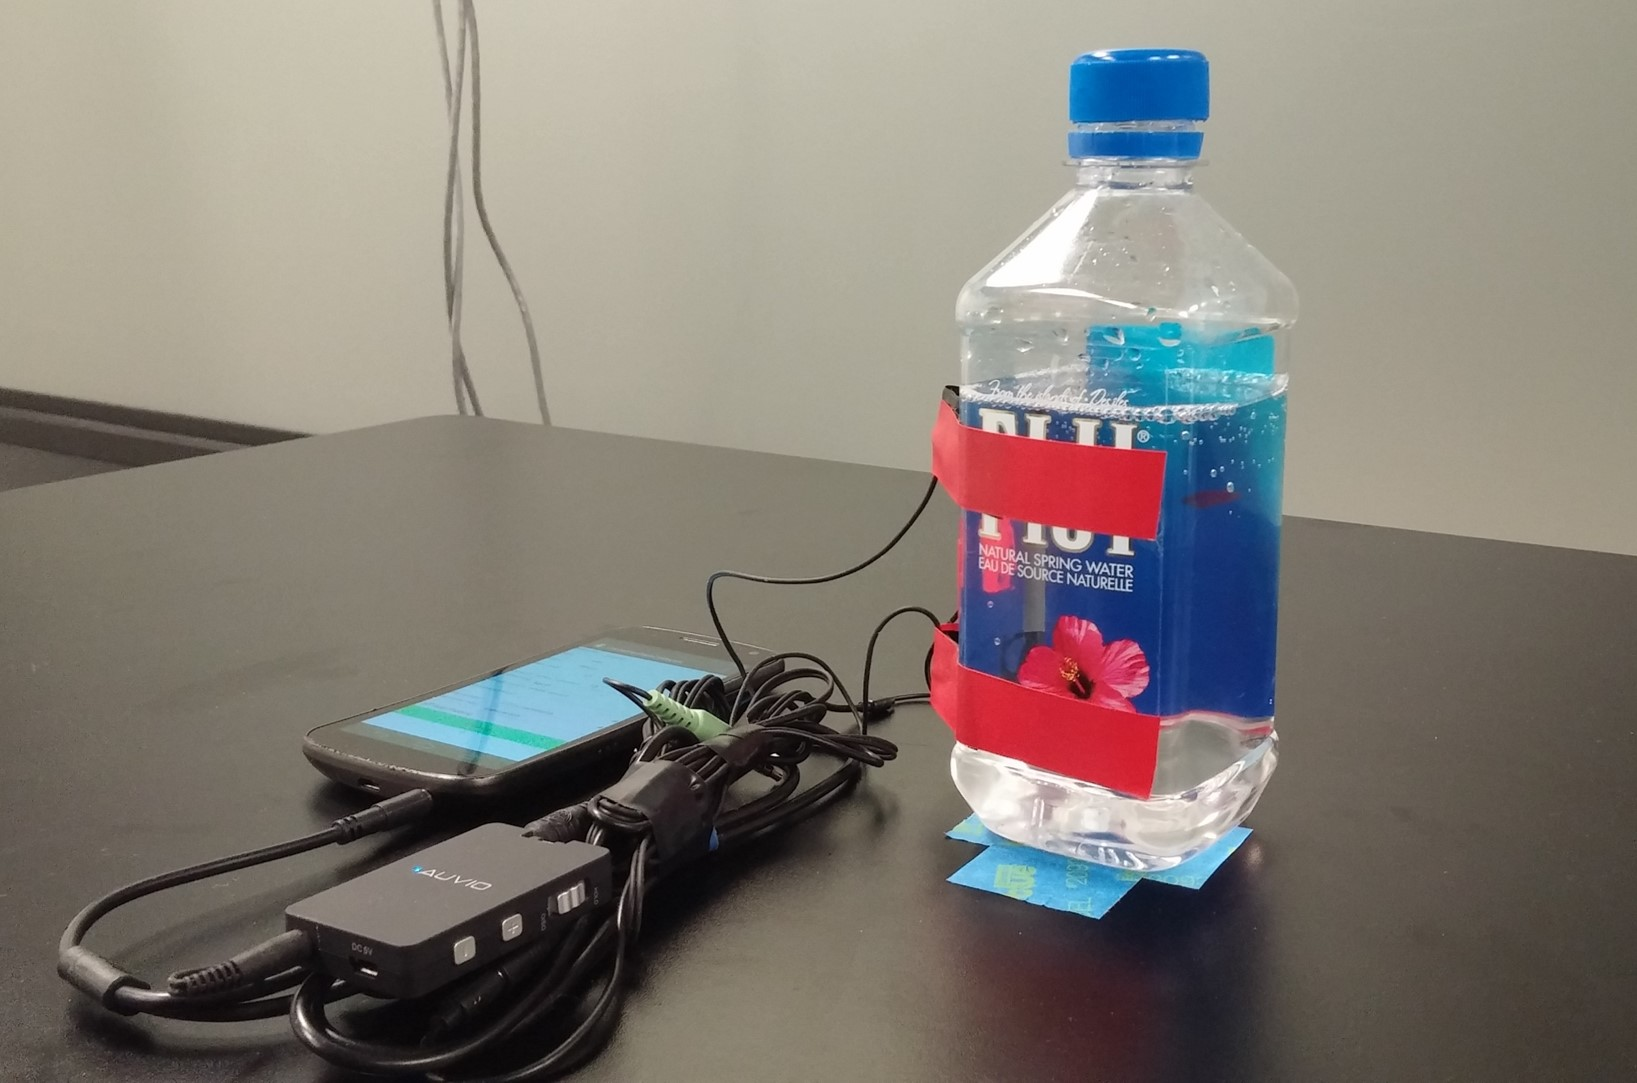
\includegraphics[width=0.5\linewidth]{setup1.jpg}
  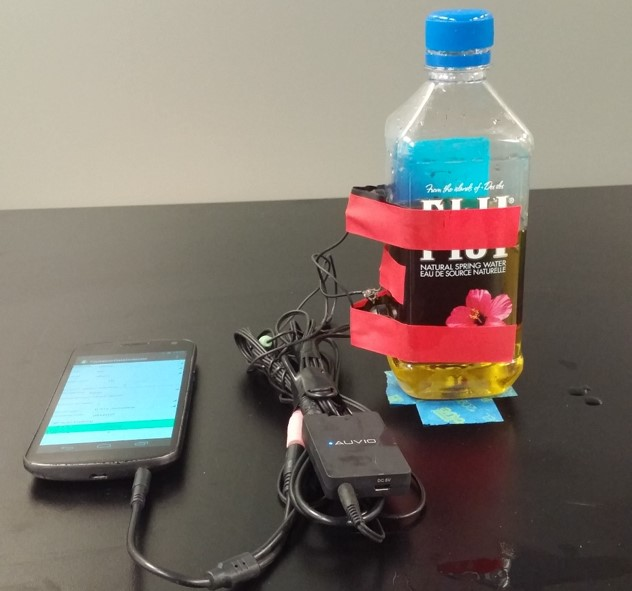
\includegraphics[width=0.242\linewidth]{setup2.jpg}
  \caption{Setup for data collection: the sensor unit is attached to a side surface of a bottle. The unit is connected to an android phone, where a data collection application runs.}
  \label{fig:set-up}
\end{figure}
\begin{figure}[htb]
\centering
\begin{subfigure}{0.32\linewidth}
  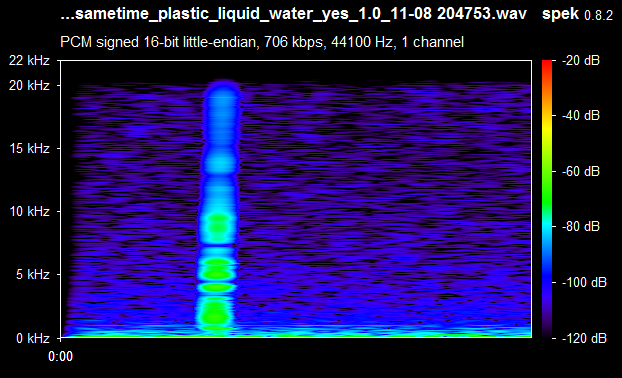
\includegraphics[width=\linewidth]{water_empty.png}
  \caption*{Empty}
\end{subfigure}
\begin{subfigure}{0.32\linewidth}
  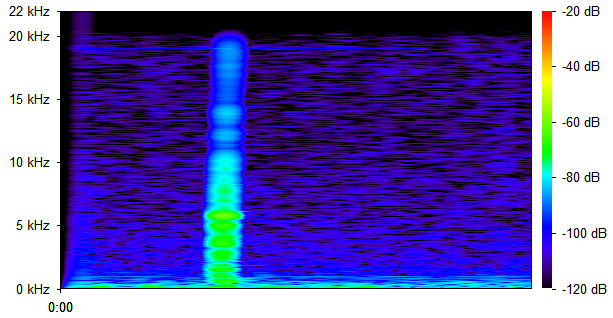
\includegraphics[width=\linewidth]{water_half.png}
  \caption*{Half-filled}
\end{subfigure}
\begin{subfigure}{0.32\linewidth}
  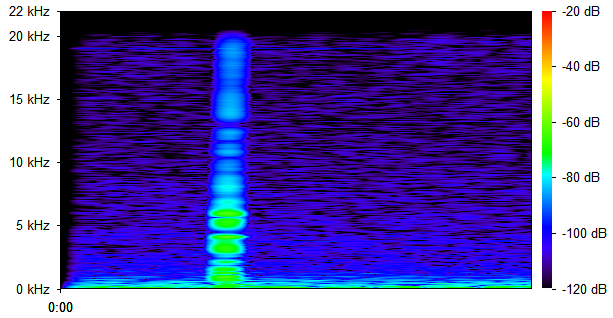
\includegraphics[width=\linewidth]{water_full.png}
  \caption*{Fully filled}
\end{subfigure}
%  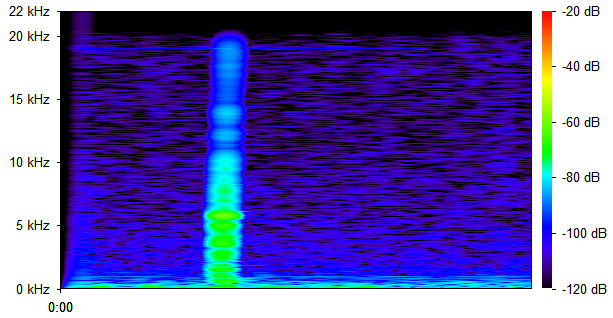
\includegraphics[width=0.3\linewidth]{water_half.png}
%  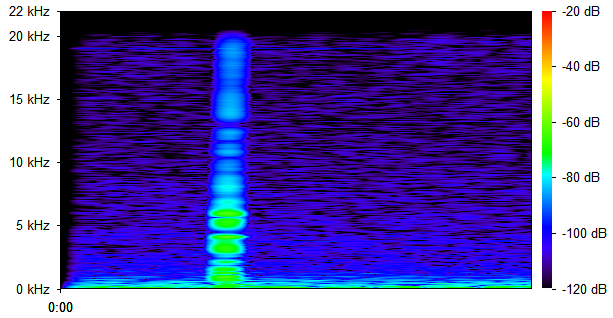
\includegraphics[width=0.3\linewidth]{water_full.png}
  \caption{Spectrograms of impulse response recordings when the bottle contains water.}
  \label{fig:set-up}
\end{figure}

We follow the same data collection protocol as we have used in our previous paper~\cite{fan2015soqr}. A brief summary of the data collection steps is presented below:

1. Choose one liquid from the 9 candidate liquid.

2. Start from the empty level. Start the mobile data collection application. The application will start probing the container and record the impulse response for 100 times.

3. After it finishes data collection for current level, we measure 10 percent of the liquid using a beak and pour the liquid into the container. We wait until the liquid settles and then start the mobile application for data collection.

4. We repeat step 3 until the container is fully filled.

5. We clean the container and start the above 1-4 steps until we finish collecting data samples for all 9 liquid.

For the data set of each liquid, there are 11 content levels in total and 100 sample audio recordings per content level. Thus, there are 1100 sample recordings per liquid and 9900 for all liquid.   

\section{Feature Extraction}
To make use of these raw audio samples, we extract and use the following two types of acoustic features: Mel-frequency cepstral coefficients (MFCCs) and linear predictive coefficients (LPC). MFCCs capture properties of the real cepstral of a short-time signal derived from the fast Fourier transform of an acoustic signal. It has been used for speech recognition and scene understanding~\cite{kunze2007symbolic}~\cite{fan2014public}, etc. LPC calculates the power spectrum of a signal and has been demonstrated efficient for formant analysis and speech analysis. 

To extract these two features, an audio recording is divided into short-time frames using a sliding window of size $W = 512$ samples and 50 percent overlap between two adjacent windows. The output frames are smoothed with a Hamming window function applied and then are converted to frequency domain via fast Fourier transformation. The magnitudes of each frequency bin $k\ (k=1\dots W)$ of a frame $j$ are represented as $\mathtt{FFT}_{j,k}$. We then identify the portion of the recording where the impulse response impacts the most by using the following equation.
\[\argmax_{i\in\{1\dots N\}}\left(\sum_{j=i}^{\min \{i+S, N\}}\sum_{K=0}^{W-1}\mathtt{FFT}_{j,k}\right)\]
where, $S$ is the number of frames during a sweep. That is, $S=(44100*0.01)/(W*50\%)$.

Finally, for the identified portion, we extract 13 MFCCs and 10 LPC for each frame, and them compute the average value of each feature. We remove the first MFCC feature because the distribution of this feature over all levels of any type of liquid are random and. We also remove the last LPC feature because it is always the same for all levels of all liquid types. Therefore, we have 21 features for learning our prediction models.

\begin{figure}
\centering
  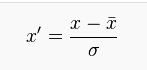
\includegraphics[width=\linewidth]{standadization_equation.PNG}
  \label{fig:equation_std}
\end{figure}

The range of raw features varies differently for different MFCCs and LPC. This might affect the optimization of our objective functions while training our prediction models. Therefore, we normalize each one of the 21 features using the following standardization equation ~\ref{fig:equation_std}.


\section{Feature Exploration}
todo: exploration and visualization of all features.

1. shows the feature change over different levels for one liquid


\section{Evaluation}
In this section, we report our exploration on the proposed research questions.

\subsection{Research Questions}
We examine the following research questions.

R1: For a given liquid, can we build a classifier that can tell its content level? This question is meant to validate the results that our previous paper has discovered using the new data set we have collected.

R2: Given N types of known liquid data and 2 levels of an unknown liquid data, could we build a model that predicts its content level? If we can build a model, how many types of known liquid we need in order to achieve a decent performance? Put it differently, we want to explore how the prediction model's performance change as the number of known liquid (N) used for training increases. 


\subsection{Exploration on R1}
The classification problem here is to predict the content level from 11 possible levels (0 to 1 with 10 percent as the interval) given the extracted 21 standardized MFCC and LPC features computed from an impulse response sound clip recorded using our sensor. We train a support vector machine classifier using libSVM~\cite{chang2011libsvm}. For evaluation, we did 10-fold cross validation. The evaluation result is shown in Table X. With the data set we collected, we were able to achieve the similar performance as ~\cite{fan2015soqr}. 

\subsection{Exploration on R2}
As the prediction class (content level) is a continuous value between 0 and 1, we can treat the prediction as regression.
  
\subsubsection{Ridge Regression}

\subsubsection{Artificial Neural Network}
Ridge Regression cannot handle the potential non-linear relation between the features and the target value. To cope with this problem, we further explored a non-linear regression model: artificial neural network. Specifically, we adopted a Multi-Layer Perceptron (MLP), which is a feed-forward artificial neural network model. By having nonlinear activation functions, MLP can distinguish the data that is not linearly separable. 

We designed an MLP with one input layer of 21 nodes, one output layer with 1 node to output the prediction result, and 2 hidden layers in between. We chose 2 hidden layers for the following reasons. We expected the nodes in the first hidden layer to learn more complex and informative features based on the input features. We expected the second hidden layers to learn the latent variables that determine the content level. In our case, the hidden variables are physical properties that could affect the sound absorption and reflection while traveling through the liquid. For the number of nodes in the first hidden layer, we chose (21 + 11)/2 for the first hidden layer (21 is the dimension of the input feature vector and 11 is the number of target values) by following the guidance of MLP design in a machine learning and data mining toolkit WEKA~\cite{hall2009weka}. It proposes the number of nodes for the hidden layer can be chose as (the number of attributes + the number of classes) / 2. For the number of nodes in the second hidden layer, we chose 4 because as we introduced earlier in the paper that there are 4 major physical properties (viscosity, specific heat, density, and temperature) that affect sound absorption and refection in liquid. To handle the non-linearity, we used a sigmoid function as the activation function. The MLP is visualized in Figure X. All the nodes in one layer are fully connected to the nodes in the next layer. The output of the final layer is the linear combination of its inputs multiplied by their weights.

We used squared-error loss function.\begin{equation} E=(f(x)-y)^2/2\end{equation} We used back-propagation algorithm, which is a fast way of computing gradients, to learn all the weights in the MLP. We used a mini-batch size of 100 while learning the weights. We also tuned the following parameters: learning rate, momentum, the number of epochs trained. Based on the empirical results, we finally set these parameters to be 0.3,0.2 and 2000.
 

\subsubsection{Evaluation Strategy}
Todo: explain the possible combinations for each case.

\subsubsection{Results}


\section{Conclusion}
todo: conclusion goes here.
%
%\subsection{Retrieval of style files}
%
%The style files for NIPS and other conference information are available on the World Wide Web at
%\begin{center}
%   \url{http://www.nips.cc/}
%\end{center}
%The file \verb+nips2015.pdf+ contains these 
%instructions and illustrates the
%various formatting requirements your NIPS paper must satisfy. \LaTeX{}
%users can choose between two style files:
%\verb+nips15submit_09.sty+ (to be used with \LaTeX{} version 2.09) and
%\verb+nips15submit_e.sty+ (to be used with \LaTeX{}2e). The file
%\verb+nips2015.tex+ may be used as a ``shell'' for writing your paper. All you
%have to do is replace the author, title, abstract, and text of the paper with
%your own. The file
%\verb+nips2015.rtf+ is provided as a shell for MS Word users.
%
%The formatting instructions contained in these style files are summarized in
%sections \ref{gen_inst}, \ref{headings}, and \ref{others} below.
%
%%% \subsection{Keywords for paper submission}
%%% Your NIPS paper can be submitted with any of the following keywords (more than one keyword is possible for each paper):
%
%%% \begin{verbatim}
%%% Bioinformatics
%%% Biological Vision
%%% Brain Imaging and Brain Computer Interfacing
%%% Clustering
%%% Cognitive Science
%%% Control and Reinforcement Learning
%%% Dimensionality Reduction and Manifolds
%%% Feature Selection
%%% Gaussian Processes
%%% Graphical Models
%%% Hardware Technologies
%%% Kernels
%%% Learning Theory
%%% Machine Vision
%%% Margins and Boosting
%%% Neural Networks
%%% Neuroscience
%%% Other Algorithms and Architectures
%%% Other Applications
%%% Semi-supervised Learning
%%% Speech and Signal Processing
%%% Text and Language Applications
%
%%% \end{verbatim}
%
%\section{General formatting instructions}
%\label{gen_inst}
%
%The text must be confined within a rectangle 5.5~inches (33~picas) wide and
%9~inches (54~picas) long. The left margin is 1.5~inch (9~picas).
%Use 10~point type with a vertical spacing of 11~points. Times New Roman is the
%preferred typeface throughout. Paragraphs are separated by 1/2~line space,
%with no indentation.
%
%Paper title is 17~point, initial caps/lower case, bold, centered between
%2~horizontal rules. Top rule is 4~points thick and bottom rule is 1~point
%thick. Allow 1/4~inch space above and below title to rules. All pages should
%start at 1~inch (6~picas) from the top of the page.
%
%%The version of the paper submitted for review should have ``Anonymous Author(s)'' as the author of the paper.
%
%For the final version, authors' names are
%set in boldface, and each name is centered above the corresponding
%address. The lead author's name is to be listed first (left-most), and
%the co-authors' names (if different address) are set to follow. If
%there is only one co-author, list both author and co-author side by side.
%
%Please pay special attention to the instructions in section \ref{others}
%regarding figures, tables, acknowledgments, and references.
%
%\section{Headings: first level}
%\label{headings}
%
%First level headings are lower case (except for first word and proper nouns),
%flush left, bold and in point size 12. One line space before the first level
%heading and 1/2~line space after the first level heading.
%
%\subsection{Headings: second level}
%
%Second level headings are lower case (except for first word and proper nouns),
%flush left, bold and in point size 10. One line space before the second level
%heading and 1/2~line space after the second level heading.
%
%\subsubsection{Headings: third level}
%
%Third level headings are lower case (except for first word and proper nouns),
%flush left, bold and in point size 10. One line space before the third level
%heading and 1/2~line space after the third level heading.
%
%\section{Citations, figures, tables, references}
%\label{others}
%
%These instructions apply to everyone, regardless of the formatter being used.
%
%\subsection{Citations within the text}
%
%Citations within the text should be numbered consecutively. The corresponding
%number is to appear enclosed in square brackets, such as [1] or [2]-[5]. The
%corresponding references are to be listed in the same order at the end of the
%paper, in the \textbf{References} section. (Note: the standard
%\textsc{Bib\TeX} style \texttt{unsrt} produces this.) As to the format of the
%references themselves, any style is acceptable as long as it is used
%consistently.
%
%As submission is double blind, refer to your own published work in the 
%third person. That is, use ``In the previous work of Jones et al.\ [4]'',
%not ``In our previous work [4]''. If you cite your other papers that
%are not widely available (e.g.\ a journal paper under review), use
%anonymous author names in the citation, e.g.\ an author of the
%form ``A.\ Anonymous''. 
%
%
%\subsection{Footnotes}
%
%Indicate footnotes with a number\footnote{Sample of the first footnote} in the
%text. Place the footnotes at the bottom of the page on which they appear.
%Precede the footnote with a horizontal rule of 2~inches
%(12~picas).\footnote{Sample of the second footnote}
%
%\subsection{Figures}
%
%All artwork must be neat, clean, and legible. Lines should be dark
%enough for purposes of reproduction; art work should not be
%hand-drawn. The figure number and caption always appear after the
%figure. Place one line space before the figure caption, and one line
%space after the figure. The figure caption is lower case (except for
%first word and proper nouns); figures are numbered consecutively.
%
%Make sure the figure caption does not get separated from the figure.
%Leave sufficient space to avoid splitting the figure and figure caption.
%
%You may use color figures. 
%However, it is best for the
%figure captions and the paper body to make sense if the paper is printed
%either in black/white or in color.
%\begin{figure}[h]
%\begin{center}
%%\framebox[4.0in]{$\;$}
%\fbox{\rule[-.5cm]{0cm}{4cm} \rule[-.5cm]{4cm}{0cm}}
%\end{center}
%\caption{Sample figure caption.}
%\end{figure}

\subsection{Tables}

All tables must be centered, neat, clean and legible. Do not use hand-drawn
tables. The table number and title always appear before the table. See
Table~\ref{sample-table}.

Place one line space before the table title, one line space after the table
title, and one line space after the table. The table title must be lower case
(except for first word and proper nouns); tables are numbered consecutively.

\begin{table}[t]
\caption{Sample table title}
\label{sample-table}
\begin{center}
\begin{tabular}{ll}
\multicolumn{1}{c}{\bf PART}  &\multicolumn{1}{c}{\bf DESCRIPTION}
\\ \hline \\
Dendrite         &Input terminal \\
Axon             &Output terminal \\
Soma             &Cell body (contains cell nucleus) \\
\end{tabular}
\end{center}
\end{table}
%
%\section{Final instructions}
%Do not change any aspects of the formatting parameters in the style files.
%In particular, do not modify the width or length of the rectangle the text
%should fit into, and do not change font sizes (except perhaps in the
%\textbf{References} section; see below). Please note that pages should be
%numbered.
%
%\section{Preparing PostScript or PDF files}
%
%Please prepare PostScript or PDF files with paper size ``US Letter'', and
%not, for example, ``A4''. The -t
%letter option on dvips will produce US Letter files.
%
%Fonts were the main cause of problems in the past years. Your PDF file must
%only contain Type 1 or Embedded TrueType fonts. Here are a few instructions
%to achieve this.
%
%\begin{itemize}
%
%\item You can check which fonts a PDF files uses.  In Acrobat Reader,
%select the menu Files$>$Document Properties$>$Fonts and select Show All Fonts. You can
%also use the program \verb+pdffonts+ which comes with \verb+xpdf+ and is
%available out-of-the-box on most Linux machines.
%
%\item The IEEE has recommendations for generating PDF files whose fonts
%are also acceptable for NIPS. Please see
%\url{http://www.emfield.org/icuwb2010/downloads/IEEE-PDF-SpecV32.pdf}
%
%\item LaTeX users:
%
%\begin{itemize}
%
%\item Consider directly generating PDF files using \verb+pdflatex+
%(especially if you are a MiKTeX user). 
%PDF figures must be substituted for EPS figures, however.
%
%\item Otherwise, please generate your PostScript and PDF files with the following commands:
%\begin{verbatim} 
%dvips mypaper.dvi -t letter -Ppdf -G0 -o mypaper.ps
%ps2pdf mypaper.ps mypaper.pdf
%\end{verbatim}
%
%Check that the PDF files only contains Type 1 fonts. 
%For the final version, please send us both the Postscript file and
%the PDF file. 
%
%\item xfig "patterned" shapes are implemented with 
%bitmap fonts.  Use "solid" shapes instead. 
%\item The \verb+\bbold+ package almost always uses bitmap
%fonts.  You can try the equivalent AMS Fonts with command
%\begin{verbatim}
%\usepackage[psamsfonts]{amssymb}
%\end{verbatim}
% or use the following workaround for reals, natural and complex: 
%\begin{verbatim}
%\newcommand{\RR}{I\!\!R} %real numbers
%\newcommand{\Nat}{I\!\!N} %natural numbers 
%\newcommand{\CC}{I\!\!\!\!C} %complex numbers
%\end{verbatim}
%
%\item Sometimes the problematic fonts are used in figures
%included in LaTeX files. The ghostscript program \verb+eps2eps+ is the simplest
%way to clean such figures. For black and white figures, slightly better
%results can be achieved with program \verb+potrace+.
%\end{itemize}
%\item MSWord and Windows users (via PDF file):
%\begin{itemize}
%\item Install the Microsoft Save as PDF Office 2007 Add-in from
%\url{http://www.microsoft.com/downloads/details.aspx?displaylang=en\&familyid=4d951911-3e7e-4ae6-b059-a2e79ed87041}
%\item Select ``Save or Publish to PDF'' from the Office or File menu
%\end{itemize}
%\item MSWord and Mac OS X users (via PDF file):
%\begin{itemize}
%\item From the print menu, click the PDF drop-down box, and select ``Save
%as PDF...''
%\end{itemize}
%\item MSWord and Windows users (via PS file):
%\begin{itemize}
%\item To create a new printer
%on your computer, install the AdobePS printer driver and the Adobe Distiller PPD file from
%\url{http://www.adobe.com/support/downloads/detail.jsp?ftpID=204} {\it Note:} You must reboot your PC after installing the
%AdobePS driver for it to take effect.
%\item To produce the ps file, select ``Print'' from the MS app, choose
%the installed AdobePS printer, click on ``Properties'', click on ``Advanced.''
%\item Set ``TrueType Font'' to be ``Download as Softfont''
%\item Open the ``PostScript Options'' folder
%\item Select ``PostScript Output Option'' to be ``Optimize for Portability''
%\item Select ``TrueType Font Download Option'' to be ``Outline''
%\item Select ``Send PostScript Error Handler'' to be ``No''
%\item Click ``OK'' three times, print your file.
%\item Now, use Adobe Acrobat Distiller or ps2pdf to create a PDF file from
%the PS file. In Acrobat, check the option ``Embed all fonts'' if
%applicable.
%\end{itemize}
%
%\end{itemize}
%If your file contains Type 3 fonts or non embedded TrueType fonts, we will
%ask you to fix it. 
%
%\subsection{Margins in LaTeX}
% 
%Most of the margin problems come from figures positioned by hand using
%\verb+\special+ or other commands. We suggest using the command
%\verb+\includegraphics+
%from the graphicx package. Always specify the figure width as a multiple of
%the line width as in the example below using .eps graphics
%\begin{verbatim}
%   \usepackage[dvips]{graphicx} ... 
%   \includegraphics[width=0.8\linewidth]{myfile.eps} 
%\end{verbatim}
%or % Apr 2009 addition
%\begin{verbatim}
%   \usepackage[pdftex]{graphicx} ... 
%   \includegraphics[width=0.8\linewidth]{myfile.pdf} 
%\end{verbatim}
%for .pdf graphics. 
%See section 4.4 in the graphics bundle documentation (\url{http://www.ctan.org/tex-archive/macros/latex/required/graphics/grfguide.ps}) 
% 
%A number of width problems arise when LaTeX cannot properly hyphenate a
%line. Please give LaTeX hyphenation hints using the \verb+\-+ command.


\subsubsection*{Acknowledgments}

Use unnumbered third level headings for the acknowledgments. All
acknowledgments go at the end of the paper. Do not include 
acknowledgments in the anonymized submission, only in the 
final paper. 


\bibliography{report}
\bibliographystyle{plain}
\end{document}
